\section{文本预处理}
在自然语言处理中,数据源处理的好坏直接影响到跑出来的模型的效果,可见,文本预处理在自然语言处理中是尤为重要的一环。对于不同语言的文本,预处理的过程是不一样的。对于英文,由于词与词之间已经用空格分隔开了,要做的只是把英文单词的时态和单复数等问题解决就行。

但是对于中文文本来说,由于词与词之间不存在间隔,无法直接分词,需要借助分词工具。同样,分词的效果好坏直接影响了聚类的效果。本章主要介绍我在中文文本预处理中执行的三大操作:名词归一化替换、中文分词、word2vec词向量化。

\subsection{非专业名词归一化替换}

在一份没有经过任何处理的法律文书中,往往充斥着大量原告被告、地名、金额、日期、数量、时间、期限、法律法条等信息,这类信息若不处理,会导致下一步的中文分词分错,进而使得聚类模型跑偏,结果不准确。
但是这类信息也是有效的,单纯地去掉也会导致关键因子的丢失,故采用替换为统一的名词来处理,比如原告名字统一替换为“原告”,金额数据统一替换为“金额”等等。

本文使用了两种方法来替换原文:一种是基于词典的替换,另一种是基于正则的替换。在网络上可以找到很全的地名字典,故可以直接用地名字典去匹配原文中的地名,然后统一替换成“地址”。

剩下的非专业名词使用正则表达式来进行替换。所用正则表达式如下:
\begin{itemize}
	\item \textbf{大数目金额}:\zihao{-4}$(([1-9]\backslash \backslash d*[\backslash \backslash d,,]*\backslash \backslash .?\backslash \backslash d*)|(0\backslash \backslash .[0-9]+))$(元|百万|万元|亿元)

	\item \textbf{原、被告名字}: \zihao{-4}$((?<=($原告|被告$)$:$).*?(?=$,$|\/|$。|、))

	\item \textbf{日期}:\zihao{-4}$\backslash$d$\{$4$\}$(年)$\backslash$d$\{$1,2$\}$(月)$\backslash$d$\{$1,2$\}$(日)|(?:$\backslash$d$\{$1,2$\}$|[$\backslash$u4e00-$\backslash$u9fa5])(?:个月|个星期|个工作日|日)|$\backslash$d$\{$4$\}$(年)$\backslash$d$\{$1,2$\}$(月)|$\backslash$d$\{$1,2$\}$(月)$\backslash$d$\{$1,2$\}$(日)|$\backslash$d$\{$4$\}$(> >
	年)|$\backslash$d$\{$1,4$\}$(日)

	\item \textbf{利息}: \zihao{-4}($\backslash$d*($\backslash$.$\backslash$d*)?(?:$\backslash$\%|%|‰))|(百|千|万)分之[$\backslash$u4e00-$\backslash$u9fa5]$\{$1,2$\}$(点[$\backslash$u4e00-$\backslash$u9fa5])?|($\backslash$d(分))

	\item \textbf{数量}: \zihao{-4}((?:$\backslash$d|[$\backslash$u4e00-$\backslash$u9fa5])(?:份|张|次))
	
	\item \textbf{期限}: \zihao{-4}(?:$\backslash$d$\{$1,2$\}$|[$\backslash$u4e00-$\backslash$u9fa5])(?:个月|个星期)|[$\backslash$u4e00-$\backslash$u9fa5]月|$\backslash$d$\{$1,3$\}$(天)
\end{itemize}

通过上述正则表达式,匹配替换原词为指定的统一词汇,可以让文本的结构更加清晰,同时又保留了这部分关键词,分词的准确率有了很大的提升。

\subsection{中文分词}
中文分词,是自然语言处理中的最基本的问题,如果中文分词不正确,中文NLP的其他算法也无法进行下去。由于中文的字与词是相连的,没有一个结构化的方法来划分,故需要一些算法来把它们分成独立的词,目前常用的分词方法有五种。

第一种是\textbf{正向最大匹配},最大正向匹配是基于词典的匹配,首先设置一个最长窗口长度。然后从句子左边开始,向右扫描,每次移动一格,若窗口内有词语出现在了词典中,则标记该词语。这种算法能在大多数情况下生效,但是一旦句子里有多义词或未登陆词\footnote{\label{unlogin_word}未登陆词:词典中未录入的词语},那这个算法将无法识别。第二种是\textbf{逆向最大匹配},这种算法原理跟正向最大匹配一样,只是窗口滑动方向是从最右边的词尾开始,滑向词头。第三种是\textbf{双向最大匹配},这个算法同时运用了正向最大匹配和逆向最大匹配,得到两种匹配的结果后对比,若两种分词的结果一样,那就认为是切分成功,采用分词结果。若两种算法的分词结果不一致,则表明出现了歧义现象或者出现了未登录词语。第四种是\textbf{N-gram双向最大匹配}。Ngram算法是基于统计的分词,他是通过计算样本的所有切分方案的概率,选择概率最大的那个。这个模型是基于一个这样的假设,一个句子中,第n个词的出现只与前面n-1个词相关,与其他句子中的词不相关。设$W_i$为句子中每个词的概率,$P \left( T \right)$为当条句子的概率,如公式\ref{ngram_approx}所示,整条句子的概率,约等于这个句子中每个词的概率的乘积。第五种是\textbf{基于隐马尔科夫模型(HMM)的分词},HMM模型主要是解决未登陆词的问题。

\begin{equation}
	\begin{aligned}
		P(T) &= P(W_1W_2W_3…W_n) \\
				&= P(W_1)P(W_2|W_1)P(W_3|W_1W_2)…P(W_n|W_1W_2…W_{n-1}) \\
				&\approx P(W_1)P(W_2|W_1)P(W_3|W_2)…P(W_n|W_{n-1})\\
	\end{aligned}
\label{ngram_approx}
\end{equation}


本文采用的是\textbf{jieba分词}的分词词工具,结巴分词主要是采用
\begin{itemize}
	\item 基于前缀的词典实现的词图扫描,对句子中的汉字的所有成词情况,生成有向无环图 (DAG)
	\item 通过动态规划来查找最大概率路径, 找到基于词频的最大切分组合
	\item 采用了HMM模型,并使用$Viterbi$算法算法优化,解决了未登陆词的问题
\end{itemize}

测试数据表明,jieba分词能正确地切分绝大多的句子,即使句子中有未登陆词,jieba分词也能正确地切分出来,在处理一些极端的情况,如“结婚的和尚未结婚的”这种句子,jieba分词也能正确地切分。


\subsection{词向量化}
经过了jieba分词的处理,我们已经把每个句子转化为词语组成的集合,但是聚类算法主要是通过计算两个向量的距离来判断两个样本的相似度,所以我们光拿词语组成的集合是不够的。还需要把词语转换成向量。

把句子转化为向量的方法大致有两种,1.通过词袋模型转换,2. 通过词向量模型转换


\subsubsection{词袋模型}
词袋模型,顾名思义也就是将所有词语装进一个袋子里,不考虑其词法和语序的问题,即每个词语都是独立的。
词袋模型最常用的方法是One-Hot Encoding,即把数据中所有词语去重后,一一映射到一个大小与去重词语数量相等的数组上,数组的每元素值都只能为0或者1,0表示映射到该下标的词语没有出现,1表示映射到该下标的词语出现了。具体例子如下

\newpage
首先给出两个简单的样本,如下所示: 

\begin{enumerate}
	\item $[$ He, is, a, male $]$
	\item $[$ She, is, a, female $]$
\end{enumerate}

根据上面两个例句,就可以构成一个词袋,袋子中含有的词为He、She、is、a、male、female,假设构建一个数组[He, She, is, a, male, female]来匹配映射,那么上面两句话可以转化成以下两组向量来表示

\begin{enumerate}
	\item $[$ 1, 0, 1, 1, 1, 0 $]$
	\item $[$ 0, 1, 1, 1, 0, 1 $]$
\end{enumerate}
	
这两个词频向量就是基于词袋模型转换出来的向量,可以看出,这样转换的坏处是语境上下文完全丢失了,只保留了单词出现的频率,这是不足以完全展示一个句子的含义。

同时,当你的词袋内的词越多,向量的维度就会越大。我在一开始做词向量化的时候用的就是词袋模型,导致我的向量的维度是十几万!这运行起来简直是个灾难,速度非常慢。所以一般我们不用原生的词袋模型来做词向量化。

\subsubsection{Word2Vec词向量模型}
那么如何有效地把切词切出来的集合转换成计算机能够识别处理的信息呢?本文使用了开源项目gensim中Word2cev模块。它是一个NLP工具,在2013年被google推出。它通过词嵌入(Word Embedding)的做法,在保存词与词的联系的前提下,把词向量的维度降到最低。从概念上来说,它是通过局部线性嵌入(LLE)来学习高维度的数据结构的低维表示方法。word2vec是基于人工神经网络的,比过去的的非监督式学习和N-Gram语法模型都要快很多。

\begin{figure}[htbp]
	\centering
	\begin{subfigure}{.5\textwidth}
		\centering
		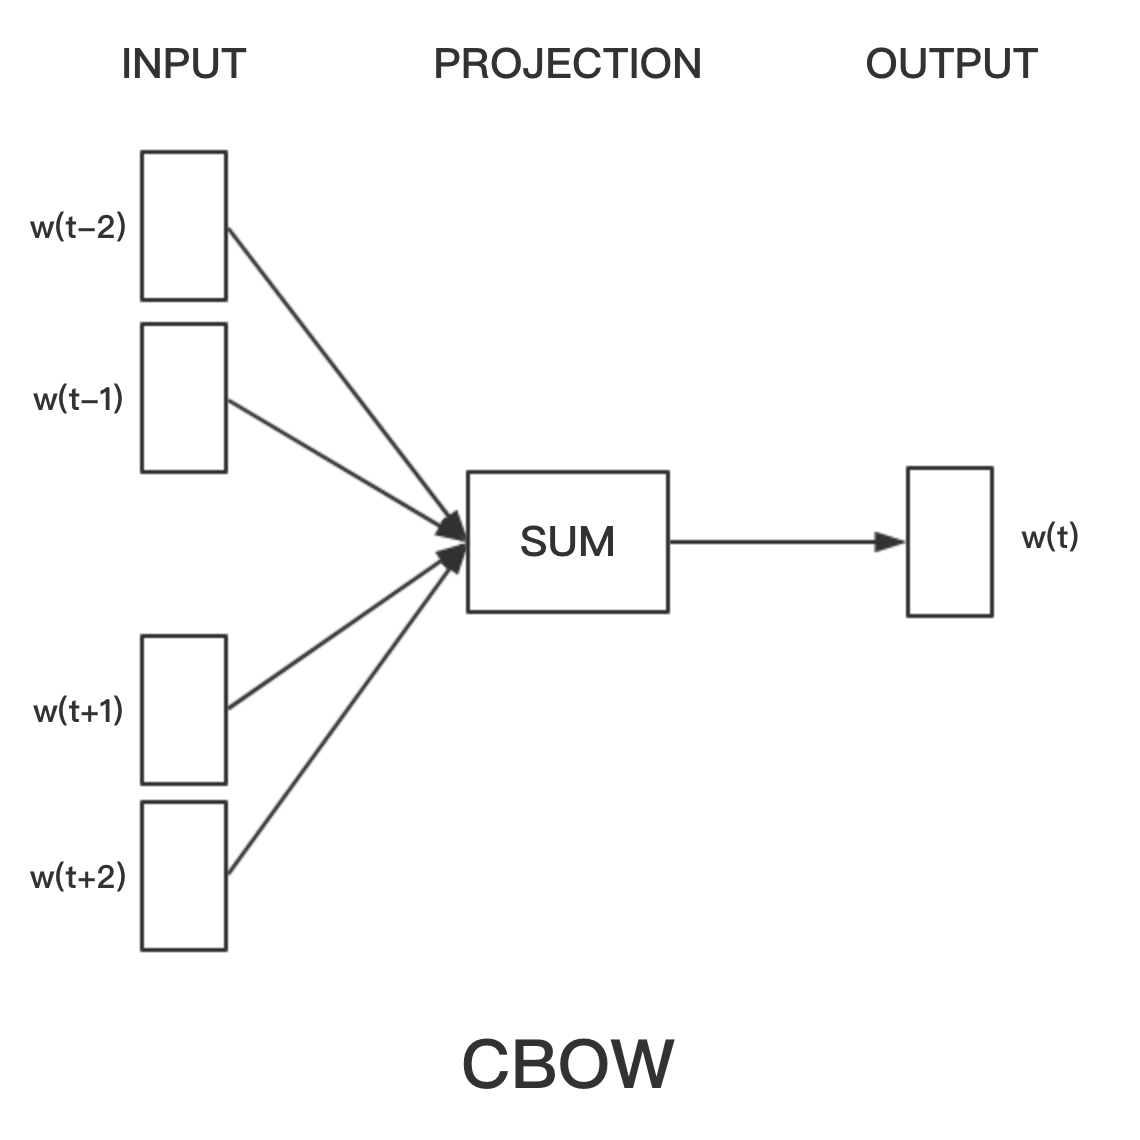
\includegraphics[width=1\linewidth]{cbow.png}
		\caption{CBOW 模型}
		\label{word_vec:cbow}
	\end{subfigure}%
	\begin{subfigure}{.5\textwidth}
		\centering
		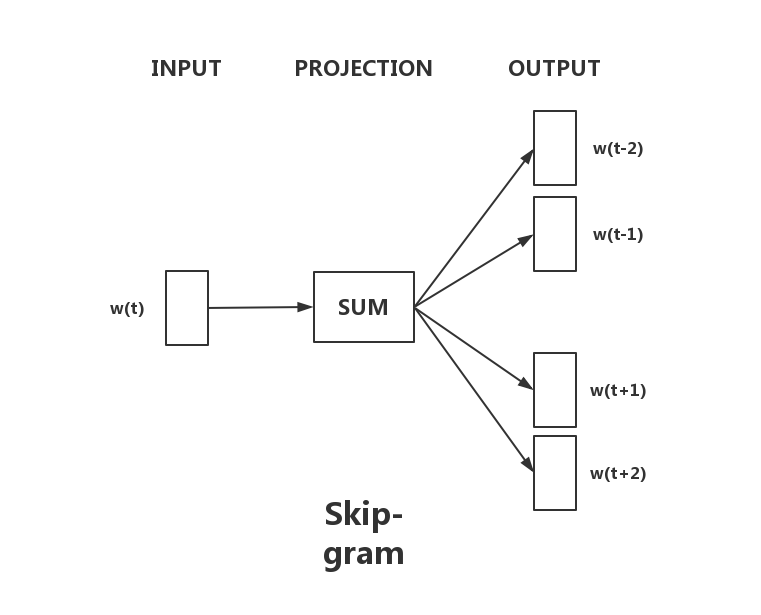
\includegraphics[width=1\linewidth]{Skip-gram.png}
		\caption{Skip-Gram 模型}
		\label{word_vec:skip_gram}
	\end{subfigure}
	\caption{词向量模型}
	\label{word_vec:example}
\end{figure}

Word2Vec里面有两个模型,CBOW模型和Skip-gram模型,如图\ref{word_vec:cbow}所示,cbow是通过词$W_t$去推断$W_t$的上下文$(W_{t+2}...W_{t-2})$, 而Skip-gram与cbow模型刚好对称,是通过$W_t$的上下文来推断$W_t$, skip-gram如图\ref{word_vec:skip_gram}所示

本项目使用了开源项目gensim的模块$gensim.models$中的\textbf{Word2vec}和$gensim.models.word2vec$中的\textbf{PathLineSentences},\textbf{Word2vec}用于训练word2vec词向量,\textbf{PathLineSentences}用于以文件流的形式逐步读取数据,以减轻内存的压力。\textbf{Word2vec}的参数如表\ref{w2v_arg_table}所示:

\begin{table}[h!]
  \begin{center}
    \renewcommand\arraystretch{1.5}
    \begin{tabular}{|cc|cc|}
      \hline
      \textbf{参数} & \textbf{说明} & \textbf{参数} & \textbf{说明} \\
			\hline
			sentence & 训练数据 & window & 包括上下文和中间词的窗口宽度 \\
			\multirow{2}*{sg} & sg=1,采用CBOW模型 & \multirow{2}*{min\_count} & \multirow{2}*{词向量中的词出现最低频次} \\
      ~ & sg=0,采用Skip-gram模型 & ~ & ~ \\
			size & 词向量的维度 & workers & 训练word2vec时调用的系统核数量 \\
			
      \hline
    \end{tabular}
    \caption{Word2vec参数取值}
    \label{w2v_arg_table}
  \end{center}
\end{table} 

\textbf{sentence:} 用于设置word2vec训练数据源,一般传一个PathLineSentences对象。PathLineSentences对象构造时接受一个参数,路径名,它会足一读取路径下的所有文档,文档的内容是要经过切词的,并且以空格分隔开,格式如图\ref{cut_word_file}所示:

\textbf{sg:} sg=0时,用Skip-gram模型进行训练,sg=1时用CBOW模型进行训练。


\begin{figure}[htbp]
  % caption放上面就会显示在图的上方,出现在下面就是出现在图的下方
  % label的位置也有讲究
  \begin{center}
    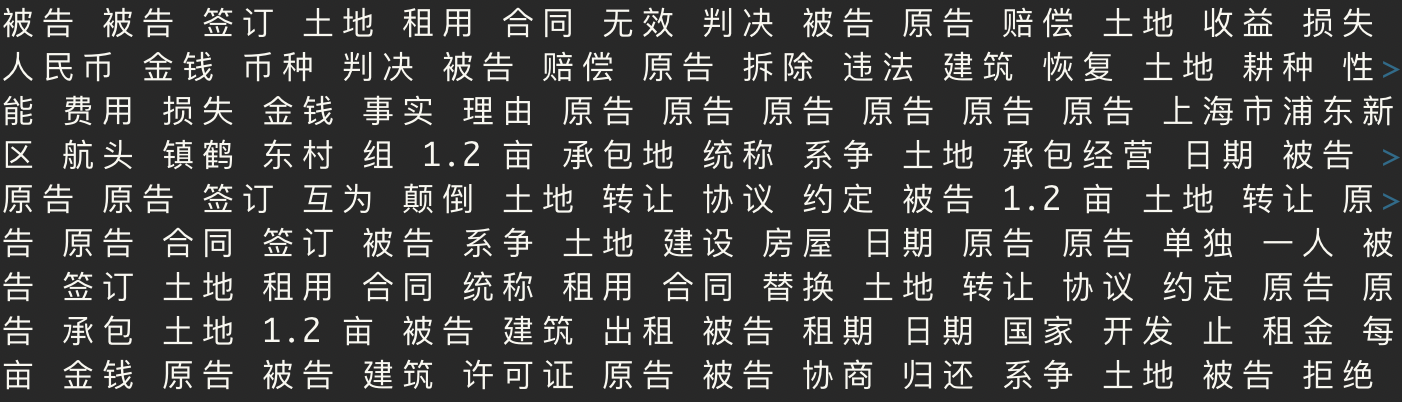
\includegraphics[width=5in]{cut_word_result.png}
    \caption{切好词的文档}
    \label{cut_word_file}
  \end{center}
\end{figure} 

